\chapter{Details}
%------------------------------------------------------------------------------
% Elaboration
%20 pages. Details of the Dependency Analysis Plugin (DAP. Describe the DAP-DB and %DAP-INCQUERY solution too. 
%------------------------------------------------------------------------------

%
\section{Infrastructure at CERN controls systems}

\subsection{Used tools}
- Describe, how a typical developer works at CERN BE-CO 
- Tools: SVN, Eclipse, Common Build, JIRA, etc. % check this at some papers of vito.

\subsection{Development workflow}
- Original idea comes from the typical development workflow lifecycle at CERN
control systems. %Insert one-by one the explanation form my thesis1 report.

% ------------------------------------------------------------------------------
% Bytecode analysis
% ------------------------------------------------------------------------------
\section{Bytecode analyzer}
% Why
Before the system performs dependency analysis, it needs to extract the
necessary information from the source code.
% What
The Bytecode analyzer module takes the input java binaries (in the form of jar
files) parses the contained class files with the help of Apache BCEL and
maps it into an object graph which can be effectively used during the dependency
processing. 
% How
\subsection{Anatomy of a Java binary}
The Bytecode analyzer module takes a set of jars as an input. A jar file is
essentially a zip file containing Java-related resources: resource files, binary
class files and meta-information. Because the system has to discover
dependencies between pure Java applications then no meta-information is used;
the bytecode analyzer gets the information from the class files contained in the
jars.

% Describe the ConstantMethodRef/FieldRef/Class/String in more details?
Figure \autoref{fig:classfile.pdf} shows a simplified view how a single class
file is built. This structure is precisely defined in Java Runtime
Specification. The class begins with a marker header followed by the part called
\textit{constant pool} which contains the textual part of the code. It contains
the i) constant strings ii) referenced methods and fields and iii) the names of
the external classes. The Java virtual machine is only able to load a class file
if all the referenced external classes are loaded.

\pic{classfile.pdf}{Internal structure of a class file}

After the constant pool the access flags, the implemented interfaces and the
field list are located in separate places.

% Describe the bytecode instructions?
Afterwards comes the definition of the methods. It contains all the necessary
information for the virtual machine to execute the methods: the resources to 
allocate for the execution, the exception handlers and the bytecode itself. 

The big question is what information can be extracted from the jar/class files
for the dependency analysis? The short answer is everything. The structure of a
class file can be obtained one-by-one. The external references what we are
looking for are also fairly easily to extract, because they are defined in the
constant pool. The only challenging part to solve is to match, where exactly are
the external resources are used in the bytecode itself.

\subsection{The analysis process}

The module extract all necessary information from the class files for processing
them. This could be done by brute-force parsing binary files, but it would be an
tedious and error-prone task. Instead of this the implementation reuses Apache
BCEL to effectively parse the class files and and to obtain the necessary
information via simple API calls.
\pic{bytecodeanal.pdf}{Steps of the bytecode analysis process}
\autoref{fig:bytecodeanal.pdf} shows the steps of the analysis process and the
related information in the class files for each step. 

The analysis starts with gathering the basic structure. This involves acquiring
the class' name, the name of the extended class and the implemented interfaces,
the defined fields and methods. This information is accessible out of the box
through the BCEL API.  

The second step is to acquire all external reference pointing outside of the
class files. For imported classes it is easy because this is what the
\code{ConstantClass} entries cover in the constant pool. For field and method
references, the implementations searches \code{ConstantFieldRef} and
\code{ConstantMethodRef} occurrences in the bytecode and saves all methods 
which uses them.

The next step is to convert the information into source format. This is
necessary because both the structure and the external references are presented
in a format which not readable nor could be easily queried by the users of the
data. For example the commonly used \code{println(String)} function has the
following binary format: \code{println(Ljava/lang/String;)V}. The implementation
transforms it into \code{println(java.lang.String):void}.

% Somewhere it should be described that we don't deal with reflection, just
% static dependencies.
The final step is to cleanup the gathered information. At this step have to
consider that if we mapped all information then the gathered data would have a
comparable size with the binary repositories which is unacceptable when we have
to deal with thousands of jars. To resolve this, the implementation does
multiple cleanup steps. First it drops the private methods and fields, because
it is not explicitly accessible and by this no dependency would point them. The
other trick is to drop a subset of the external references. The
platform-provided elements are dropped (references pointing inside the
\code{java.*} package) and the ones which point inside the jar files. This is
reasonable because any IDE gives access this information through code traversal
capabilities. Of course this cleanup needs do be done after all class files are 
parsed in a jar file. 


\subsection{Extracted domain model}
The output of the analyzer is a java domain model.
\picr{domainmodelsimp.pdf}{Classes of the domain model used by the bytecode analyzer}
\autoref{fig:domainmodelsimp.pdf} shows the elements of this model. Because this model
is used for the dependency processing too the model has additional elements which is 
now not important. 

All element inherits from abstract \code{CodeElement} class which is a top-level
interface for handing the items of the model. The processed jar files are named
as \code{Product}s, because that's what it is: a software product. A product
contains several classes named \code{ApiClass} which store the class-level
properties. The required classes are stored in the \code{referencedClasses}
list. The classes contain some \code{Field}s and some \code{Method}s which both have 
a -- source formatted -- signature and some access properties. The \code{referencedFields}
and the \code{referencedMethods} hold all the external field and method references which are
accessed or invoked in the bytecode of the represented method. 

With an instance of this domain model the dependency processing module is capable of 
discovering the dependency relationships between certain parts of the dependency.
 
 
 
\section{Dependency processor}
- Sequence, how the dependency analysis works. 
- Summarize what should be found if execute the analysis in the example
\begin{figure}[htb]                                            
   \center   
   \caption{Sequence of bytecode analysis} 
   \label{fig:analization.pdf}  
     \resizebox{0.7\linewidth}{!}{
      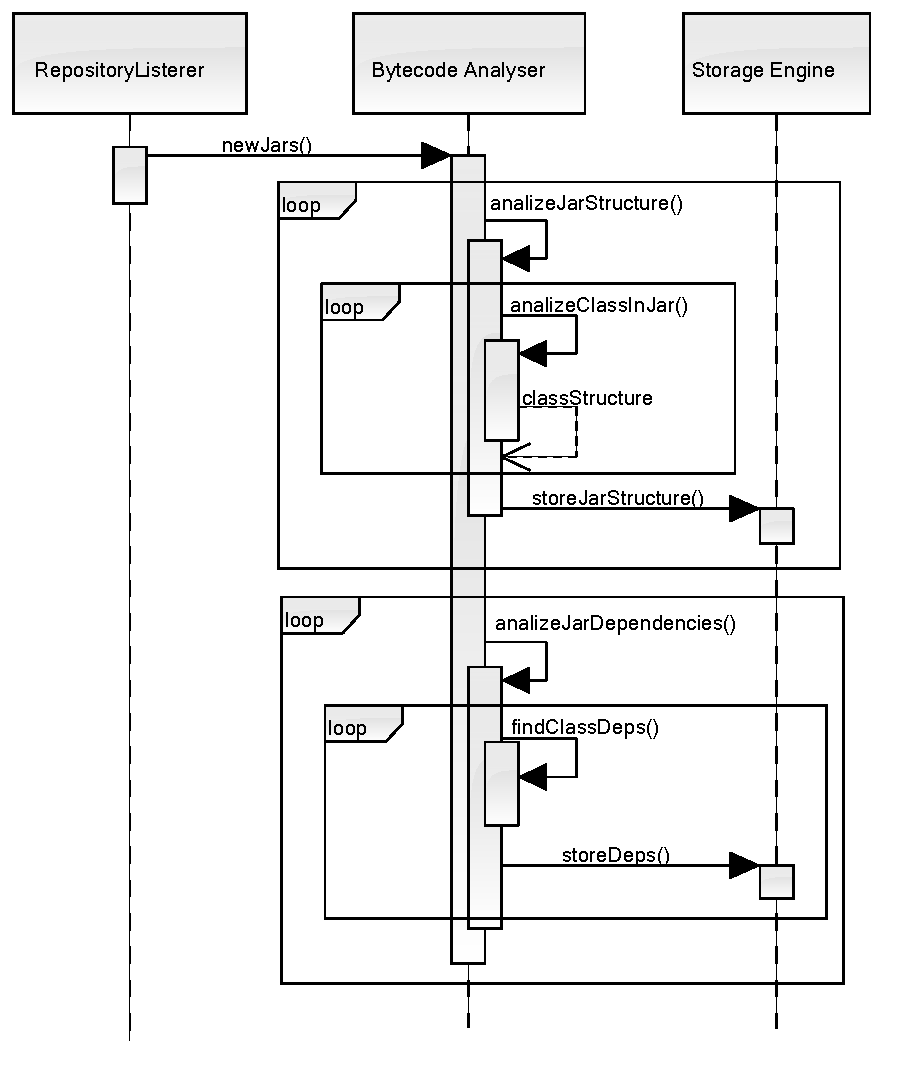
\includegraphics{figures/analization.pdf}
      } 
\end{figure}

%------------------------------------------------------------------------------
% Persistence
%------------------------------------------------------------------------------
\section{Persisting dependencies} 
- describe the saved domain model.
- describe the how the operations work:
 * store structure
 * find and insert dependencies
- introduce different implementation 
- the result 

\section{Direct queries}
- Explain eclipse plugin; ui contribution.
- Simple workflow: right click on source code->jdt resolves it as a
class-method-field-> fully qualify it -> sends the query for the server process
-> the process returns the incoming dependencies depending the passed type. ->
the result is visualized in a view.
- Show it on the example: what if the developer wants to change the the
signature of a service function OR what if he wants to change the name of the
name of the default provider name.

\section{Repository EMF model}
% bonus: retrieve the model to the client

\section{Creation of workspace EMF model}
- Java Model representation in Eclipse. 
- Dependency search in Eclipse.
- EMF model generation:
 * How to obtain the structure 
 * How to obtain internal dependency environment
 * and how to listen to changes.

\section{Pattern matching}
- Mention again that the source code and the repository contains the same information. (+svn tags)
- How to obtain more precise information.
- The repository model. 
- Describing the queries.
* joining the two implementation. 
* incoming dependencies
* impact analysis
  * added and removed methods
  * removed methods
  * changed methods: the outgoing dependency set has new elements, which does not exist in the repo model. 
-  Show it on the example.
